\documentclass[a4paper,11pt]{article}
\usepackage[margin=0.8in]{geometry}
\usepackage{xcolor}
\usepackage{graphicx} %package to manage images
\graphicspath{ {./images/} }
\usepackage{multicol}
\usepackage{float}
\usepackage{amsmath}

\title{1.3.4 Web Technologies}
\author{Revision sheet}
\date{}

\usepackage{fancyhdr}
\pagestyle{fancy}
\fancyhead{} % clear all header fields
\renewcommand{\headrulewidth}{0pt} % no line in header area
\fancyfoot{} % clear all footer fields
\renewcommand{\footrulewidth}{0.4pt}
\fancyfoot[C]{\thepage} % page number in centre of the page
\fancyfoot[R]{\footnotesize Thomas Boxall \\ } % right hand footer has author name on top line and images reference on bottom line
\fancyfoot[L]{\footnotesize 1.3.4 Web Technologies \\ Revision sheet} % left hand footer has title of document on top line and 'Revision Sheet' on bottom line


\begin{document}

\maketitle
\thispagestyle{fancy}

% CONTENTS OF THE REVISION SHEET HERE
\begin{multicols}{2}
\section{Web Programming}
See separate \textit{Web Development Languages} document.

\section{Search Engine Indexing}
Search engines use databases (also known as an index) of web pages to find the pages which a user is looking for. To build the index, a piece of software called a \textit{web crawler} or \textit{spider} is used. Different search engines use different algorithms, however fundamentally they start with pages currently in the index then use hyperlinks from those pages to find other web pages which they don't have in their index; these are added to the index and the algorithm starts again, with new pages this time. 
\subsection{Search Engine Results}
There are a number of different elements which can be used by the search engine to index what is on the page. Meta tags (\verb|<meta>| allow keywords or descriptions of the web pages to be added. Search engines can then use this to point users at pages which mach their search criteria. The meta tags go within the head element of a HTML page. The headings and titles of web pages are also used, these are usually a good indication of the content on the website. 
\subsection{Google's PageRank Algorithm}
The PageRank algorithm was introduced to solve the problem of unreliable rankings in search engines. It used the number of links linking into that page as well as number of links linking away from that page to determine the rank. Factors such as who produced the content were also taken into consideration, for example pages with \verb|.gov| domains would rank higher. The web was represented as a directed graph, with every web page being a node, hyperlinks as edges and the PageRank value as the weighting on the edges.

\section{PageRank Algorithm}
The PageRank algorithm has the following formula:\\
$\displaystyle PR(A) = (1-d) + d \left(\displaystyle \frac{PR(T_1)}{C(T_1)} + ... + \frac{PR(T_n)}{C(T_n)} \right)$\\
where
\begin{itemize}
    \item $PR(A)$ is the PageRank of page A.
    \item $C(T_n)$ is the total count of outbound links from web page $n$ including the inbound links to page A. 
    \item $\frac{PR(T_n}{C(T_n}$ is the share of the vote that page A gets from $T_1 ... T_n$. Each of these fractions is added together then the total is multiplied by $d$.
    \item $d$ is the damping factor, which is used to prevent $\frac{PR(T_1)}{C(T_1)}$ from having too much influence. It is set to a value of $0.85$, which accounts for a user clicking through 6 web pages before leaving the website or entering a new web address.
\end{itemize}
The PageRank algorithm has to be applied in multiple iterations so that values can be adjusted appropriately, as other pages PageRank values are also calculated. Usually three is a suitable number of times to repeat the algorithm.
\end{multicols}
\section{PageRank Example}
The example below shows how the PageRank algorithm would be applied to the following set of web pages (A, B, C and D).
\begin{figure}[H]
    \centering
    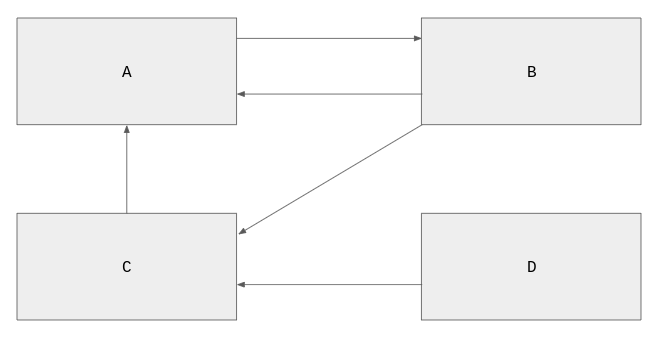
\includegraphics[width=0.9\textwidth]{images/PageRankExample.png}
    \caption{Example web pages}
    \label{fig:pageRankExample}
\end{figure}
\subsection{Iteration I}
\begin{align*}
    PR(A) &= (1-d) + d \left(\frac{PR(B)}{2} + \frac{PR(C)}{1}\right) &&= (1-0.85) + 0.85 \left(\frac{1}{2} + \frac{1}{1} \right) &&&=&&& 1.425\\
    PR(B) &= (1-d) + d \left(\frac{PR(A)}{1} \right) &&= (1-0.85) + 0.85 \left(\frac{1.425}{1} \right) &&&=&&& 1.361\\
    PR(C) &= (1-d) + d \left(\frac{PR(B)}{2} + \frac{PR(D)}{1} \right) &&= (1-0.85) + 0.85 \left(\frac{1.361}{2} + \frac{1}{1} \right) &&&=&&& 1.578 \\
    PR(D) &= (1-d) + d\left(0 \right) &&= (1-0.85) + 0.85 \left(0 \right) &&&=&&& 0.15 
\end{align*}
\subsection{Iteration II}
\begin{align*}
    PR(A) &= (1-d) + d \left(\frac{PR(B)}{2} + \frac{PR(C)}{1}\right) &&= (1-0.85) + 0.85 \left(\frac{1.361}{2} + \frac{1.578}{1} \right) &&&=&&& 2.07\\
    PR(B) &= (1-d) + d \left(\frac{PR(A)}{1} \right) &&= (1-0.85) + 0.85 \left(\frac{2.07}{1} \right) &&&=&&& 1.909\\
    PR(C) &= (1-d) + d \left(\frac{PR(B)}{2} + \frac{PR(D)}{1} \right) &&= (1-0.85) + 0.85 \left(\frac{1.909}{2} + \frac{0.15}{1} \right) &&&=&&& 1.089 \\
    PR(D) &= (1-d) + d\left(0 \right) &&= (1-0.85) + 0.85 \left(0 \right) &&&=&&& 0.15 
\end{align*}
\subsection{Iteration III}
\begin{align*}
    PR(A) &= (1-d) + d \left(\frac{PR(B)}{2} + \frac{PR(C)}{1}\right) &&= (1-0.85) + 0.85 \left(\frac{1.909}{2} + \frac{1.089}{1} \right) &&&=&&& 1.887\\
    PR(B) &= (1-d) + d \left(\frac{PR(A)}{1} \right) &&= (1-0.85) + 0.85 \left(\frac{1.887}{1} \right) &&&=&&& 1.754\\
    PR(C) &= (1-d) + d \left(\frac{PR(B)}{2} + \frac{PR(D)}{1} \right) &&= (1-0.85) + 0.85 \left(\frac{1.754}{2} + \frac{0.15}{1} \right) &&&=&&& 1.023 \\
    PR(D) &= (1-d) + d\left(0 \right) &&= (1-0.85) + 0.85 \left(0 \right) &&&=&&& 0.15 
\end{align*}

\begin{multicols}{2}
\section{Client And Server Side Processing}
Using the Client-Server model, data can either be processed on the client side or on the server side. 
\subsection{Web Servers}
Clients can send request messages to web servers which should interpret the data and send an appropriate response back to the client. This might either be data which the client has requested or an error message. This is commonly seen in online travel booking forms, where the request is the search parameters and the response is the tickets which have been found.
\subsection{Client Side Processing}
Data is processed on the client computer rather than the server. This could be because the client has specific software which can process the information or to lighten the load on the servers processor. This can also improve security as it avoids unnecessary data transmission. JavaScript is a client-side language which can be used to validate data or adjust the content side to suit different devices or displays.
\subsection{Server Side Processing}
Servers process data on behalf of multiple clients. They process the data much faster than a client can and there are specific languages used for server side processing (for example, PHP or SQL). Any database queries have to be done on the server side.
\subsection{API}
An \textit{Application Protocol Interface} is a set of protocols that governs how two applications should interact with each other. It sets out the formats of requests and responses between a client and a server, allowing one application to make uses of the services of another. 
\subsection{Thick and Thin Clients}
This refers to the amount of processing the client does. The more processing that the client does (rather than the server doing it), the thicker the client becomes. 
\subsubsection{Thin Clients}
\textbf{Advantages: }Easy to set up, maintain and add terminals with very little installation required locally; software and updates can be installed on the server and automatically distributed to each client terminal; more secure since all data is kept centrally in once place. \newline
\textbf{Disadvantages: }Reliant on the server (therefore if it goes down then everything goes down); requires powerful server which is expensive; server demand and bandwidth increased; maintaining network connections for portable devices consumes more battery than local data processing.
\subsubsection{Thick Clients}
\textbf{Advantages: }Robust and reliable (gives greater up-time); can operate without a continuous connection to the server; generally better for running more powerful software applications.\newline
\textbf{Disadvantages: }More expensive, higher spec client devices required; installation of software required on each client separately (increases administration time); potential issues with data integrity once it enters a client terminal.




\end{multicols}
\end{document}

t(a) HTML, CSS and JavaScript. See appendix 5d.
t(b) Search engine indexing.
t(c) PageRank algorithm.
(d) Server and client side processing.